\title{User Manual}
\def \documentid {LEANOS-UVIE-UM-001}
\date{Issue 0.1, May 1, 2017}

\newcommand\affil[1]{\textsuperscript#1}

\def\preparedby {Armin Luntzer\affil{1}}
\def\checkedby {Roland Ottensamer\affil{1}}
\def\approvedby {Franz Kerschbaum\affil{1}}

\def\affiliations{
	\affil{1} Department of Astrophysics, University of Vienna
}




\documentclass{report}
%\usepackage[left = 2cm, right=2cm, top = 1cm]{geometry}
\usepackage[top = 2cm, bottom = 5cm]{geometry}

\usepackage[T1]{fontenc}
\usepackage{textcomp}

%\PassOptionsToPackage{table}{xcolor}


\usepackage{geometry}
\usepackage{fontspec}
%
\defaultfontfeatures[MyriadPro-SemiCondensed]{
	Path		= ../shared/fonts/,
	Extension	= .otf,
	UprightFont	= *-light,
	ItalicFont	= *-italic,
	BoldFont	= *-bold,
	BoldItalicFont	= *-bold-italic
%	LetterSpace	= 5pt		% Laufweite
}
%
\defaultfontfeatures[MyriadPro]{
	Path		= ../shared/fonts/,
	Extension	= .otf,
	UprightFont	= *-regular,
	ItalicFont	= *-italic,
	BoldFont	= *-bold,
	BoldItalicFont	= *-bold-italic
}%
\defaultfontfeatures[MyriadProLight]{
	Path		= ../shared/fonts/,
	Extension	= .otf,
	UprightFont	= MyriadPro-light,
	ItalicFont	= MyriadPro-light-italic,
}

\setmainfont{MyriadPro}



\makeatletter
\renewcommand\normalsize{%
\@setfontsize\normalsize{11pt}{14pt}
\abovedisplayskip 10\p@ \@plus2\p@ \@minus5\p@%
\abovedisplayshortskip \z@ \@plus2\p@%
\belowdisplayshortskip 5\p@ \@plus2\p@ \@minus3\p@%
\belowdisplayskip \abovedisplayskip%
\let\@listi\@listI%
}
\normalsize  
\makeatother



\usepackage{titlesec}

\titleformat{\chapter}[hang]
  {\fontspec{MyriadProLight}\fontsize{30}{36}\selectfont\color{uvie-blue}}
  {\fontspec{MyriadPro}\selectfont\thechapter.}{8pt}{}
\titlespacing*{\chapter}{0pt}{-20pt}{20pt}

\titleformat{\section}
  {\fontspec{MyriadPro}\fontsize{13}{16}\selectfont\color{uvie-blue}}
  {\thesection}{1em}{}

\titleformat{\subsection}
  {\fontspec{MyriadPro}\fontsize{13}{16}\selectfont\color{uvie-blue}}
  {\thesection}{1em}{}

\DeclareMathSizes{12}{55}{15}{15}

\usepackage[table]{xcolor}

% begin UVIE primary colours
\iffalse

% colours from numeric colour values in corporate design document
\definecolor{uvie-blue}{RGB}{0, 99, 166}
\definecolor{uvie-orangered}{RGB}{221, 72, 20}
\definecolor{uvie-goldenyellow}{RGB}{234, 171, 0}
% UVIE secondary colours
\definecolor{uvie-gray}{RGB}{102, 102, 102}
\definecolor{uvie-burgundy}{RGB}{167, 28, 73}

\else
% colours from actual colour samples in corporate design document
%r: 0 g:58 b:133
\definecolor{uvie-blue}{RGB}{0, 79, 150}
\definecolor{uvie-orangered}{RGB}{225, 55, 15}
\definecolor{uvie-goldenyellow}{RGB}{248, 169, 0}
% UVIE secondary colours
\definecolor{uvie-gray}{RGB}{104, 104, 104}
\definecolor{uvie-burgundy}{RGB}{141, 22, 51}

\fi
% end UVIE primary colours


% allowed UVIE logo height
\newlength{\maxlogoheight}\setlength{\maxlogoheight}{20mm}
\newlength{\medlogoheight}\setlength{\medlogoheight}{15mm}
\newlength{\minlogoheight}\setlength{\minlogoheight}{10mm}
%
% allowed space round logo: logoheight <= x <= 0.5 logoheight 
\def \maxlogospacing{1.0}
\def \medlogospacing{0.75}
\def \minlogospacing{0.5}

%
%elif \paperheight \equal {210mm} % A5
% todo: based on papersize: >= A4: 20mm, A5/long: 15mm, all smaller: 10mm
%\if \paperheight \equal {297mm}	  % A4
\newlength{\logoheight}{\setlength{\logoheight}{\maxlogoheight}
%elif \paperheight \equal {210mm} % A5
%\fi
%
% todo: pass as option
\newlength{\logospacing}{\setlength{\logospacing}{\medlogospacing\logoheight}


\newcommand{\fig}[1]{Figure \ref{#1}}


\newenvironment{keywords}%
   {\begin{trivlist}\item[]{\bfseries\sffamily Schlagworte:}\ }% oder "Keywords:"
   {\end{trivlist}}
%
\author{%
    Author 1 name \\
    Department name \\
    \texttt{email1@example.com}\vspace{40pt} \\
    Author 2 name \\
    Department name \\
    \texttt{email2@example.com}
    }


\usepackage{tabu}
\usepackage{colortbl}

\usepackage{array, ltxtable}
\usepackage[most]{tcolorbox}


\usepackage[some]{background}
\usepackage{tikz}
\backgroundsetup{
scale=1,
angle=0,
opacity=1,
placement=top,
contents={
	\begin{tikzpicture}[remember picture, blend mode = multiply]
		% field heights from top down: x | x | x/2 | remainder
		%
		\fill[white]		(-0.5\paperwidth,                 0.0)
							rectangle (0.5\paperwidth,       -3.0\logospacing);
		\fill[uvie-blue!75]	(-0.5\paperwidth,                -3.0\logospacing)
							rectangle (0.5\paperwidth, -2.0 * 3.0\logospacing);
		\fill[uvie-blue]	(-0.5\paperwidth,          -2.0 * 3.0\logospacing)
							rectangle (0.5\paperwidth, -2.5 * 3.0\logospacing);
		% mext can be image or colour, but must overlap with 3rd bar in multiply
		% blend mode
		% todo: make conditional on image option
		\fill[uvie-blue!75]	(-0.5\paperwidth,          -2.0 * 3.0\logospacing)
							rectangle (0.5\paperwidth,       -1.0\paperheight);
	\end{tikzpicture}}
}
%


\makeatletter
\let\doctitle\@title
\makeatother

\makeatletter
\let\docdatever\@date
\makeatother

\usepackage{fancyhdr}
\usepackage{lastpage}

\def\ifalogo{
\includegraphics[height = \medlogoheight]{../shared/images/uni_logo_astrophysik_cmyk.eps}}
\fancypagestyle{plain}{ % call style plain so it is used by chapter pages as well
	\fancyhf{}
	\fancyhead[R]{
		\fontspec{MyriadPro}\docdatever \\
		\vspace{2em}
		Page \thepage\ of \pageref*{LastPage} 
	}

	\fancyhead[C]{
		{
			\fontspec{MyriadPro}
			\documentid \\
			\vspace{.7em}
			\doctitle
			\vspace{.9em}
		}
	}
	\fancyhead[L]{
		\ifalogo%
	}
}
\setlength\headheight{80pt}
\pagestyle{plain}


% def \preparedby, \checkedby, \approvedby, \documentid, \docdatever, \doctitle
\def\approvalpage{
	\clearpage
	\pagestyle{empty}
	\null
	\vfil

	{\fontspec{MyriadPro}\fontsize{20}{24}\selectfont\color{uvie-blue}
	 \doctitle}

	\vspace*{1\baselineskip}

	\begin{tabular}{@{}ll}
		\textbf{Reference:}   & \documentid \\[2ex]
		\textbf{Version:}     & \docdatever \\[6ex]
		\textbf{Prepared by:} & \preparedby \\[1ex]
		\textbf{Checked by:}  & \checkedby  \\[1ex]
		\textbf{Approved by:} & \approvedby \\[1ex]
	\end{tabular}

	\vspace*{0.5\baselineskip}
	{\footnotesize \affiliations}


	\vfill

	\begin{minipage}[b]{0.9\textwidth}
	\footnotesize\raggedright
	\setlength{\parskip}{0.5\baselineskip}
	Copyright \copyright \the\year\ \par
	Permission is granted to copy, distribute and\slash or modify this
	document under the terms of the GNU Free Documentation License,
	Version 1.3 or any later version published by the Free Software
	Foundation; with no Front-Cover, no Logos of the University of Vienna.
	\end{minipage}
	\vspace*{2\baselineskip}
	\cleardoublepage

	\pagestyle{plain}
}

\newcommand{\uvietitlepage}[3]{%
\begin{titlepage}
\BgThispage
%
%
\begin{tikzpicture}[overlay, remember picture]
\node[anchor	= north west,
      xshift	= \logospacing,
      yshift	=-\logospacing] 
      at (current page.north west)
     {
\includegraphics[height = \logoheight]{../shared/images/uni_logo_astrophysik_cmyk.eps}}; 
\end{tikzpicture}
%
\begin{tikzpicture}[overlay, remember picture]
\node[anchor	= north east,
      xshift	=-\logospacing,
      yshift	=-\logospacing] 
      at (current page.north east)
     {
\includegraphics[height = \logoheight]{../shared/images/uni_logo_farbe_02.eps}}; 
\end{tikzpicture}
%
%
%
% main title, must not exceed 3 lines 
\begin{tikzpicture}[overlay, remember picture]
\node[anchor			= north west,
      xshift			= \logospacing,
      yshift			=-\logospacing * 3.0,
	  minimum height	= \logospacing * 3.0,
	  text width		= \textwidth]
      at (current page.north west)
      {\fontsize{30pt}{36pt}\selectfont
       \textcolor{white}
       {
			\uppercase{#1}
       }
       \par
      };
\end{tikzpicture}
%
% subtitle, must not exceed 3 lines 
\begin{tikzpicture}[overlay, remember picture]
\node[anchor			= north west,
      xshift			= \logospacing,
      yshift			=-\logospacing * 5.5,
	  minimum height	= \logospacing * 2.5,
	  text width		= \textwidth]
      at (current page.north west)
      {\fontsize{13pt}{16pt}\selectfont
       \textcolor{white}
       {
			\uppercase{\textbf {#2}}
       }
       \par
      };
\end{tikzpicture}
%
%\noindent
%\hfill
% \hspace*{-3cm}
\begin{tikzpicture}[overlay, remember picture]
\node[anchor=south east,		%anchor is upper left corner of the graphic
      xshift  = 0.5cm,		%shifting around
      yshift  = -0.5cm] 
     	at (current page.south east) %left upper corner of the page
     {\includegraphics[width=14.0cm]{#3}}; 
\end{tikzpicture}
%
%
\end{titlepage}
%
\restoregeometry
%
\newpage
}% newcommand uvietitlepage

\usepackage[xindy, nopostdot, numberedsection, style=super, section, toc, acronyms, nogroupskip]{glossaries}
\usepackage{xparse}

\setlength{\glsdescwidth}{0.8\textwidth}
\renewcommand{\glsnamefont}[1]{\textbf{#1}}

% label, acronym, name, description
\DeclareDocumentCommand{\newdualentry}{ m m m m } {
	\newglossaryentry{gls-#1}{
	name={#3 (\gls{#1})},
	description={#4}, nonumberlist
	}
	\newglossaryentry{#1}{
		type=\acronymtype,
		name={#2},
		first={#3 (#2)},
		firstplural={#3s (#2s)},
		see={[Glossary:]{\gls{gls-#1}}},
		description=\glslink{gls-#1}{#3},
		nonumberlist
	}%
}
%%% \gls{ABBREV} to point at Acronym/Abbreviation index
%%% \gls{gls-ABBREV} to point to glossary


\newdualentry{ADC}%
  {ADC}%
  {Analog to Digital Converter}%
  {An Analog to Digital Converter is a system that converts an analog signal
   into a quantized digital signal. Its counterpart is the \gls{DAC}.}%

\newdualentry{API}%
  {API}%
  {Application Programming Interface}%
  {The Application Programming Interface defines how a developer can write
   a program that requests services from an operating system or application.
   \glspl{API} are implemented by function calls composed of verbs and nouns,
   i.e. a function to execute on an object.}%

\newdualentry{BSP}%
  {BSP}%
  {Board Support Package}%
  {A Board Support Package is the implementation of a specific interface defined
   by the abstract layer of an operating system that enables the latter to run
   on the particular hardware platform.}%

\newdualentry{CPU}%
  {CPU}%
  {Central Processing Unit}%
  {The Central Processing Unit is the electronic circuitry that interprets
  instructions of a computer program and performs control logic, arithmetic,
  and input/output operations specified by the instructions. It maintains
  high-level control of peripheral components, such as memory and other devices.}%

\newdualentry{DAC}%
  {DAC}%
  {Digital to Analog Converter}%
  {A Digital to Analog Converter is a system that converts a quantized digital
   signal into an analog signal. Its counterpart is the \gls{ADC}.}%

\newdualentry{DMA}%
  {DMA}%
  {Direct Memory Access}%
  {Direct Memory Access is a feature of a computer system that allows hardware
   subsystems to access main system \gls{gls-RAM} directly, thereby bypassing
   the \gls{gls-CPU}.}%

\newdualentry{DSP}%
  {DSP}%
  {Digital Signal Processor}%
  {A Digital Signal Processor is a specialised processor with its architecture %
   targeting the operational needs of digital signal processing.}%

\newdualentry{ELF}%
  {ELF}%
  {Executable and Linkable Format}%
  {The Executable and Linkable Format is a common standard file format for
   executables, object code, shared libraries, and core dumps.}%

\newdualentry{FIFO}%
  {FIFO}%
  {First In - First Out}%
  {In FIFO processing, the "head" element of a queue is processed first.
   Once complete, the element is removed and the next element in line becomes
   the new queue head.}%

\newdualentry{FPU}%
  {FPU}%
  {Floating Point Unit}%
  {A co-processor unit that specialises in floating-point calculations.}%

\newdualentry{ILP}%
  {ILP}%
  {Instruction Level Parallelism}%
  {Instruction-level parallelism (ILP) is a measure of how many instructions in
   a computer program can be executed simultaneously by the \gls{CPU}.}%

\newdualentry{ISR}%
  {ISR}%
  {Interrupt Service Routine}%
  {An Interrupt Service Routine is a function that handles the actions needed
   to service an interrupt.}%

\newdualentry{GCC}%
  {GCC}%
  {GNU Compiler Collection}%
  {The GNU Compiler Collection is a compiler system produced by the
   GNU project. It is part of the GNU toolchain collection of programming
   tools.}%

\newglossaryentry{GNU}{
  name={GNU},
  description={GNU is a recursive acronym that stands for "GNU's Not Unix!".
	      The GNU project is a free software collaboration project announced
	      in 1987. Users are free to run GNU-licensed software, share, copy,
	      distribute, study and modify it. GNU software guarantees these
	      freedom-rights legally via its license and is thefore free
      	      software.},
  nonumberlist
}

\newglossaryentry{LEON2}{
  name={LEON2},
  description={The LEON2 is a synthesisable VHDL model of a 32-bit processor
	       compliant with the SPARC V8 architecture. It is highly
	       configurable and particularly suitable for \gls{SoC} designs.
	       Its source code is available under the GNU LGPL license},
  nonumberlist
  }

\newglossaryentry{LEON3}{
  name={LEON3},
  description={The LEON3 is an updated version of the \gls{LEON2}, changes
	       include \gls{gls-SMP} support and a deeper instruction pipeline},
  nonumberlist
  }

\newglossaryentry{LEON3-FT}{
  name={LEON3-FT},
  description={The LEON3-FT is a fault-tolerant version of the \gls{LEON3}.
  	       Changes to the base version include autonomous error handling,
       	       cache locking and different cache replacement strategies.},
  nonumberlist
  }

\newdualentry{MMU}%
  {MMU}%
  {Memory Management Unit}%
  {A Memory Management Unit performs address space translation between physical
   and virtual memory pages and protects unprivileged access to certain memory
   regions.}%

\newdualentry{MPPB}%
  {MPPB}%
  {Massively Parallel Processor Breadboarding system}%
  {The Massively Parallel Processor Breadboarding system is a proof-of-concept %
   design for a space-hardened, fault-tolerant multi-DSP system with various %
   subsystems to build a powerful digital signal processing system with a high %
   data throughput. Its distinguishing features are the \gls{gls-NoC} and the
   \gls{Xentium} \glspl{DSP} controlled by a \gls{LEON2} processor.
   It was developed under ESA contract 21986 by Recore Systems B.V.}%

\newdualentry{NGAPP}%
  {NGAPP}%
  {Next Generation Astronomy Processing Platform}%
  {Next Generation Astronomy Processing Platform was an evaluation of the
   \gls{MPPB} performed in a joint effort of RUAG Space Austria and the
   Department of Astrophysics of the University of Vienna.
   The project was funded under ESA contract 40000107815/13/NL/EL/f.}%

\newdualentry{NoC}%
  {NoC}%
  {Network On Chip}%
  {A Network On Chip is a communication system on an integrated circuit that
   applies (packet based) networking to on-chip communication. It offers
   improvements over more conventional bus interconnects and is more scalable
   and power efficient in complex \gls{gls-SoC} desgins.}%

\newdualentry{POSIX}
  {POSIX}
  {Portable Operating System Interface}
  {The Portable Operating System Interface is a family of standards specified
   by the IEEE Computer Society for maintaining compatibility between
   operating systems.}%

\newdualentry{PUS}
  {PUS}
  {Packet Utilisation Standard}
  {The Packet Utilisation Standard addresses the end-to-end transport of telemetry
   and telecommand data between user applications on the ground and applications
   onboard a satellite. See also ECSS-E-70-41A.}%

\newdualentry{RAM}%
  {RAM}%
  {Random-Access Memory}%
  {Random-Access Memory is a type of memory where each memory cell may be
   accessed directly via their memory addresses.}%

\newdualentry{RISC}%
  {RISC}%
  {Reduced Instruction Set Computing}%
  {RISC is a \gls{CPU} design strategy that intends to improve performance by
   combining a simplified instruction set with a microprocessor architecture
   that is capable of executing an instruction in a smaller number of clock
   cycles.}%

\newdualentry{RMAP}%
  {RMAP}%
  {Remote Memory Access Protocol}%
  {The Remote Memory Access Protocol is a form of \gls{SpaceWire} communication
   that transparently communicates writes to memory mapped regions between
   different hardware devices.}%


\newdualentry{RR}%
  {RR}%
  {Round Robin}%
  {Round Robin is a scheduling algorithm where time slices are assigned in equal
   poritions and in circular order. In the context of threads, priorities are
   usually only used to control re-scheduling order when a mutex is accessed by
   a thread.}%

\newacronym{RSA}{RSA}{RUAG Space Austria}

\newdualentry{SMP}%
  {SMP}%
  {Symmetric Multiprocessing}%
  {Symmetric Multiprocessing denotes computer architectures, where two or more
   identical processors are connected to the same periphery and are controlled
   by the same operating system instance.}%

\newdualentry{SoC}%
  {SoC}%
  {System On Chip}%
  {A System On Chip is an integrated circuit that combines all components of a %
   computer or other electronic system into a single chip.}%

\newglossaryentry{SpaceWire}{
  name={SpaceWire},
  description={SpaceWire is a spacecraft communication network based in part
               on the IEEE 1355 standard of communications.},
  nonumberlist
  }

\newglossaryentry{SPARC}{
  name={SPARC},
  description={SPARC ("scalable processor architecture") is a \gls{gls-RISC}
  	       instruction set architecture developed by Sun Microsystems in
	       the 1980s. The distinct feature of SPARC processors is the high
	       number of \gls{gls-CPU} registers that are accessed similarly to
	       stack variables via ``sliding windows''.},
  nonumberlist
  }

\newdualentry{SSDP} % label
  {SSDP}            % abbreviation
  {Scalable Sensor Data Processor}  % long form
  {The Scalable Sensor Data Processor (SSDP) is a next generation on-board %
   data processing mixed-signal ASIC, envisaged to be used in future scientific %
   payloads requiring high-performance on-board processing capabilities. %
   It is built opon a heterogeneous multicore architecture, combining two %
   \gls{Xentium} \gls{DSP} cores with a general-purpose \gls{LEON3-FT} control %
   processor in a \gls{gls-NoC}.} % description


\newdualentry{TCM}%
  {TCM}%
  {Tightly-Coupled Memory}%
  {Tightly-Coupled Memory is the local data memory that is directly accessible %
   by a Xentium's load/store unit. It can be viewed as a completely %
   program-controlled data cache.}%


\newacronym{UVIE}{UVIE}{University of Vienna}

\newdualentry{VLIW}%
  {VLIW}%
  {Very Long Instruction Word}%
  {Very Long Instruction Word is a processor architecture design concept that
   exploits \gls{gls-ILP}. This approach allows higher performance at a smaller
   silicone footprint compared to serialised instruction processors, as no
   instruction re-ordering logic to exploit superscalar capabilities of the
   processor must be integrated on the chip, but requires either code to be
   tuned manually or a very sophisticated compiler to exploit the full potential
   of the processor.}%

\newglossaryentry{Xentium}{
  name={Xentium},
  description={The Xentium is a high performance \gls{gls-VLIW} \gls{DSP} core.
               It operates 10 parallel execution slots supporting 32/40 bit
	       scalar and two 16-bit element vector operations.},
  nonumberlist
  }


% do not remove
\glsresetall
\makeglossaries


\usepackage{vhistory}

\usepackage{biblatex}
\addbibresource{../shared/bibliography.bib}

\usepackage{listings}

\lstdefinestyle{customc}{
  belowcaptionskip=1\baselineskip,
  breaklines=true,
  xleftmargin=\parindent,
  language=C,
  showstringspaces=false,
  basicstyle=\footnotesize\ttfamily,
  keywordstyle=\bfseries\color{uvie-orangered!75},
  commentstyle=\itshape\color{uvie-gray},
  identifierstyle=\color{uvie-blue},
  stringstyle=\color{uvie-goldenyellow},
}

\usepackage{appendix}

%% use pageref instead of pageref*, the latter only works
%% for cross-document referencing (architecture/requirements)
%% need to find a more universial solution at some point
\fancypagestyle{plain}{ % call style plain so it is used by chapter pages as well
	\fancyhf{}
	\fancyhead[R]{
		\fontspec{MyriadPro}\docdatever \\
		\vspace{2em}
		Page \thepage\ of \pageref{LastPage} 
	}

	\fancyhead[C]{
		{
			\fontspec{MyriadPro}
			\documentid \\
			\vspace{.7em}
			\doctitle
			\vspace{.9em}
		}
	}
	\fancyhead[L]{
		\ifalogo%
	}
}

\begin{document}
\lstset{style=customc} 


\setmainfont{MyriadPro-SemiCondensed}
\uvietitlepage%
{Lean OS --\\ An operating system for the SSDP}%
{\doctitle}%
{../shared/images/logo2.pdf}
\setmainfont{MyriadPro}

\approvalpage

\tableofcontents
\newpage



\begin{versionhistory}
  \vhEntry{0.1}{01.05.2017}{AL}{Initial version}
\end{versionhistory}


\chapter{Introduction}

\section{Purpose of the Document}

This document gives an overview on how to use the LeanOS operating system.

\chapter{Applicable and Reference Documents} % does not break automatically for some reason

\printbibliography[heading=none]


\chapter{Terms, Definitions and Abbreviated Items}
\printglossary[type=acronym]
\printglossary[type=main, style=altlist]



\chapter{Software Overview}

\section{Function and Purpose}

This software is an operating system targeting in particular the use of the
Xentium DSPs found in \glspl{SoC} like the \gls{SSDP} or \gls{MPPB}.
\\

The source code components are split into architecture-specific and generic
sources that depend on the implementation of certain interfaces by the former.
While this means that any architecture could be supported, the only
currently implemented hardware architecture is SPARC/LEON.

%%\section {How to get LeanOS}

\section {Build Requirements}

In order to build LeanOS, make sure you have set up your environment variables
to point to the compilers to be used. You will need at least a cross-compiler
for the \gls{SPARC} platform (i.e. BCC from Gaisler or SPARC GCC from RECORE)
and a \gls{GCC} compiler for your host platform. In addition, you will need
also need GNU make, appropriate versions of binutils and a bash shell, i.e.
what you would typically find in a Linux distribution with a basic set of
development and system tools installed. If you want to generate source code
documentation, you will also need to install \gls{Doxygen}. To generate
documents from LaTeX source files, you will also need an appropriate TeX
environment.

\section {Build System}

LeanOS uses an adaptation of the Linux kernel's Kbuild system. For details on
how to use it, you may refer to related documentation found online. \\

\noindent
To launch the configuration interface, simply issue 

\begin{lstlisting}[language=bash]
  $ make menuconfig
\end{lstlisting}
\noindent
on your shell prompt from the top-level LeanOS directory. If you prefer a
graphical interface, you may use:

\begin{lstlisting}[language=bash]
  $ make gconfig
\end{lstlisting}

\noindent
You can now configure the build as you desire. The menu items are usually
descriptive, but if you are unsure, have a look at the help text of an item for
more information. Note that some options may only appear if a certain
prerequisite has been enabled, i.e. unless you check \emph{Enable
System-On-Chip Configurations} and do not select the correct CPU target, you
will not be able to build for the \gls{SSDP} or the \gls{MPPB}.  You will also
not be able to select any of the specific drivers, e.g. for the \gls{NoC}
\gls{DMA}. Once you are satisfied with your selection, save and exit the
configuration interface.\\

\noindent
To build a kernel image, you can now issue

\begin{lstlisting}[language=bash]
  $ make
\end{lstlisting}

\noindent
on your command line. The build process will produce an executable ELF binary
named \emph{leanos} which you can then run on your target system using your
preferred method, e.g. via grmon.



\section {Source and Support Documentation}

To generate source code documentation in HTML, go to \emph{Documentation/doxygen}
and run \emph{make}.

To render support documents such as this one from their LaTeX sources, go
to \emph{Documentation/doxygen} and follow the instructions in the README file.




\section {Xentium Kernel Programs}

To build \gls{Xentium} processing kernels, you must install the Xentium
development tools (available from RECORE) in your path and select the
configuration option \emph{Build Xentium DSP kernel programs}.  If you have
configured loadable module support and embedded image generation (see below),
the generated Xentium kernel will be automatically embedded in your kernel
image and loaded on boot. \\

\noindent
The source code to the Xentium programs is located in the \emph{dsp/}
subdirectory.


\section {Xentium Processing Demo}

To build a LeanOS kernel that demonstrates a Xentium processing network setup,
select \emph{Enable System-On-Chip configurations}, then configure your CPU and
board type (LEON2/3, MPPB/SSDP). In the submenu \emph{System-on-Chip
drivers}, enable the \emph{NoC 2D DMA driver} and \emph{Xentium processing
network support}, but make sure to set them to \emph{built-in} if you have
enabled loadable module support. Now select \emph{Build Xentium DSP kernel
programs} and \emph{Build a Xentium Processing Demo kernel} in the main menu,
then \emph{make} the kernel image.

\section {Sample Code}

Use the configuration interface to enable and select sample code to be built.
Run

\begin{lstlisting}[language=bash]
  $ make samples
\end{lstlisting}

\noindent
to build the executables. They will be placed in the \emph{samples/}
subdirectories.



\section {Features Overview}

The following will give you a concise overview of some of the currently 
implemented features of LeanOS that distinguish it from other operating
systems in its class.

\subsection {Memory Management}

A fully working \emph{malloc}/\emph{free} interface has been implemented on top
of lower-tier page/chunk allocators with optional SPARC SRMMU support.
SRMMU-based page mapping is done on-demand (i.e. lazy mapping). Situations
where the operating system runs out of physical memory are detected, but
currently no action is taken except to halt the system. This can be easily
extended to boot into safe mode or take other FDIR measures when a faulty
software configuration uses physical memory above a critical threshold.

\subsection {Loadable Modules}

The operating system is able to dynamically load/unload modules to extend
or patch its capabilities at run time. Modules are unlinked ELF object files.
Relocations are computed during load. Modules may also compiled into the kernel.

\subsection {Payload Images}

The kernel can interpret and load the contents of AR (archive) files. Configured
loadable modules and Xentium programs are automatically added to an archive
that is embedded into the kernel image during build. The image may also hold
arbitrary data, e.g. calibration files.


\subsection {Xentium and NoC support}

LeanOS supports the Network-on-Chip and its core features (such as the DMA)
found in the \gls{SSDP} and the \gls{MPPB}. A major focus is the integration
of the \gls{Xentium} \glspl{DSP} into a processing network that can be used to
create arbitrary pipelines on a per-task-packet basis (see below).



\chapter{Processing Networks in LeanOS}

\section{Overview}

In contrast to a typical implementation of processing pipeline, the approach
taken in this implementation is not a static route, but one that is defined
arbitrarily on a per-task basis from a set of \emph{processing kernel} nodes
consisting of small \gls{Xentium} \gls{ELF} binaries that are registered to the
operating system's \gls{Xentium} \gls{DSP} driver. Each of these nodes define
their own capability as an \emph{op code} which is read by the driver and used
to identify and set up individual processing steps of a given processing task.
\\

\noindent
To define a processing chain, the user selects a sequence of operations to be
performed on a data buffer. It is up to the user to make sure that the
processing kernels are designed in such a way, that the data format may be
interpreted properly.
A processing task is inserted into the input node of the Xentium
processing network and then autonomously passed on to all nodes in series until
it reaches the output node, where it is handed back to the user. The node
selection from the registered set of \gls{Xentium} kernels is performed by the
driver, which takes care of scheduling tasks.
\\

\noindent The concept and function of a proccessing network is described in the
following section. It is based on a generic implementation that will be
described first, followed by the specific variant for the \gls{Xentium}. Note
that it is laid out in order of dependency of the individual components, i.e.
bottom-up.



\section{Processing Tasks}

\begin{figure}
\begin{center}
	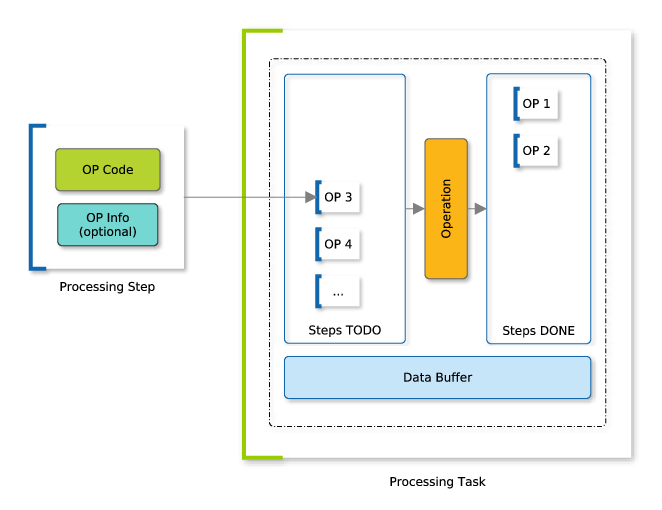
\includegraphics[width=0.7\columnwidth]{images/proc_task}
	\caption{The structure of a single processing task. Steps from the
	TODO list are moved to the DONE list of steps when the
	operation is complete. The data buffer holds the data the operations are
	performed on.}
	\label{fig:proc_task}
\end{center}
\end{figure}

A \emph{processing task} (\fig{fig:proc_task}) is the lowest-tier element of a
\emph{processing network}. It consists of a data buffer and a list of
\emph{processing steps} to perform. Optionally, a task type identifier and a
sequence number can be assigned that may be used to track tasks as part of the
user implementation of a network. Processing steps are added by configuring the
\emph{op code} of the operation to perform and optionally setting an arbitrary
data pointer associated with the particular operation. As operations are
completed on the data, the operation step record is moved from the pending
(TODO) to the completed (DONE) steps list.


\section{Processing Trackers}

\begin{figure}%[htb]
\begin{center}
	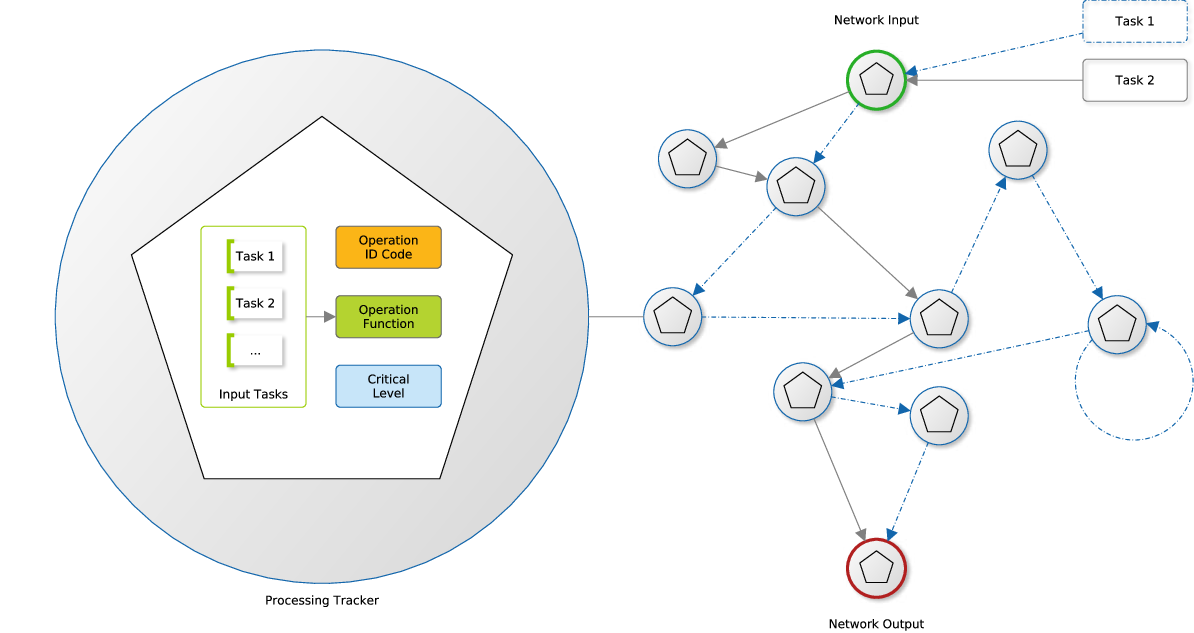
\includegraphics[width=1.0\columnwidth]{images/task_network}
	\caption{A single processing tracker node holds an op code identifier
		and a processing function. It stores an arbitrary number of
		tasks at its input. A critical level defines a threshold above
		which the pending tasks in a tracker should be preferred for
		processing. Multiple task tracker nodes form a processing
		network. Tasks inserted into the network propagate through
		nodes on arbitary paths or even multiple times (as defined by
		their processing step list) through the same node unti they
		reach the output node.}
	\label{fig:task_network}
\end{center}
\end{figure}

In order to processs the tasks fed into the network, nodes must be created,
which execute the desired processing steps listed in the task.  These nodes are
the \emph{processing trackers} (\fig{fig:task_network}). Each processing
tracker is initialised with an op code and a function to execute the particular
operation. Trackers have a property called the \emph{critical level}, which is
the treshold of pending input tasks above which a tracker should be processed
with priority.


\section{Processing Networks}


\begin{figure}%[htb]
\begin{center}
	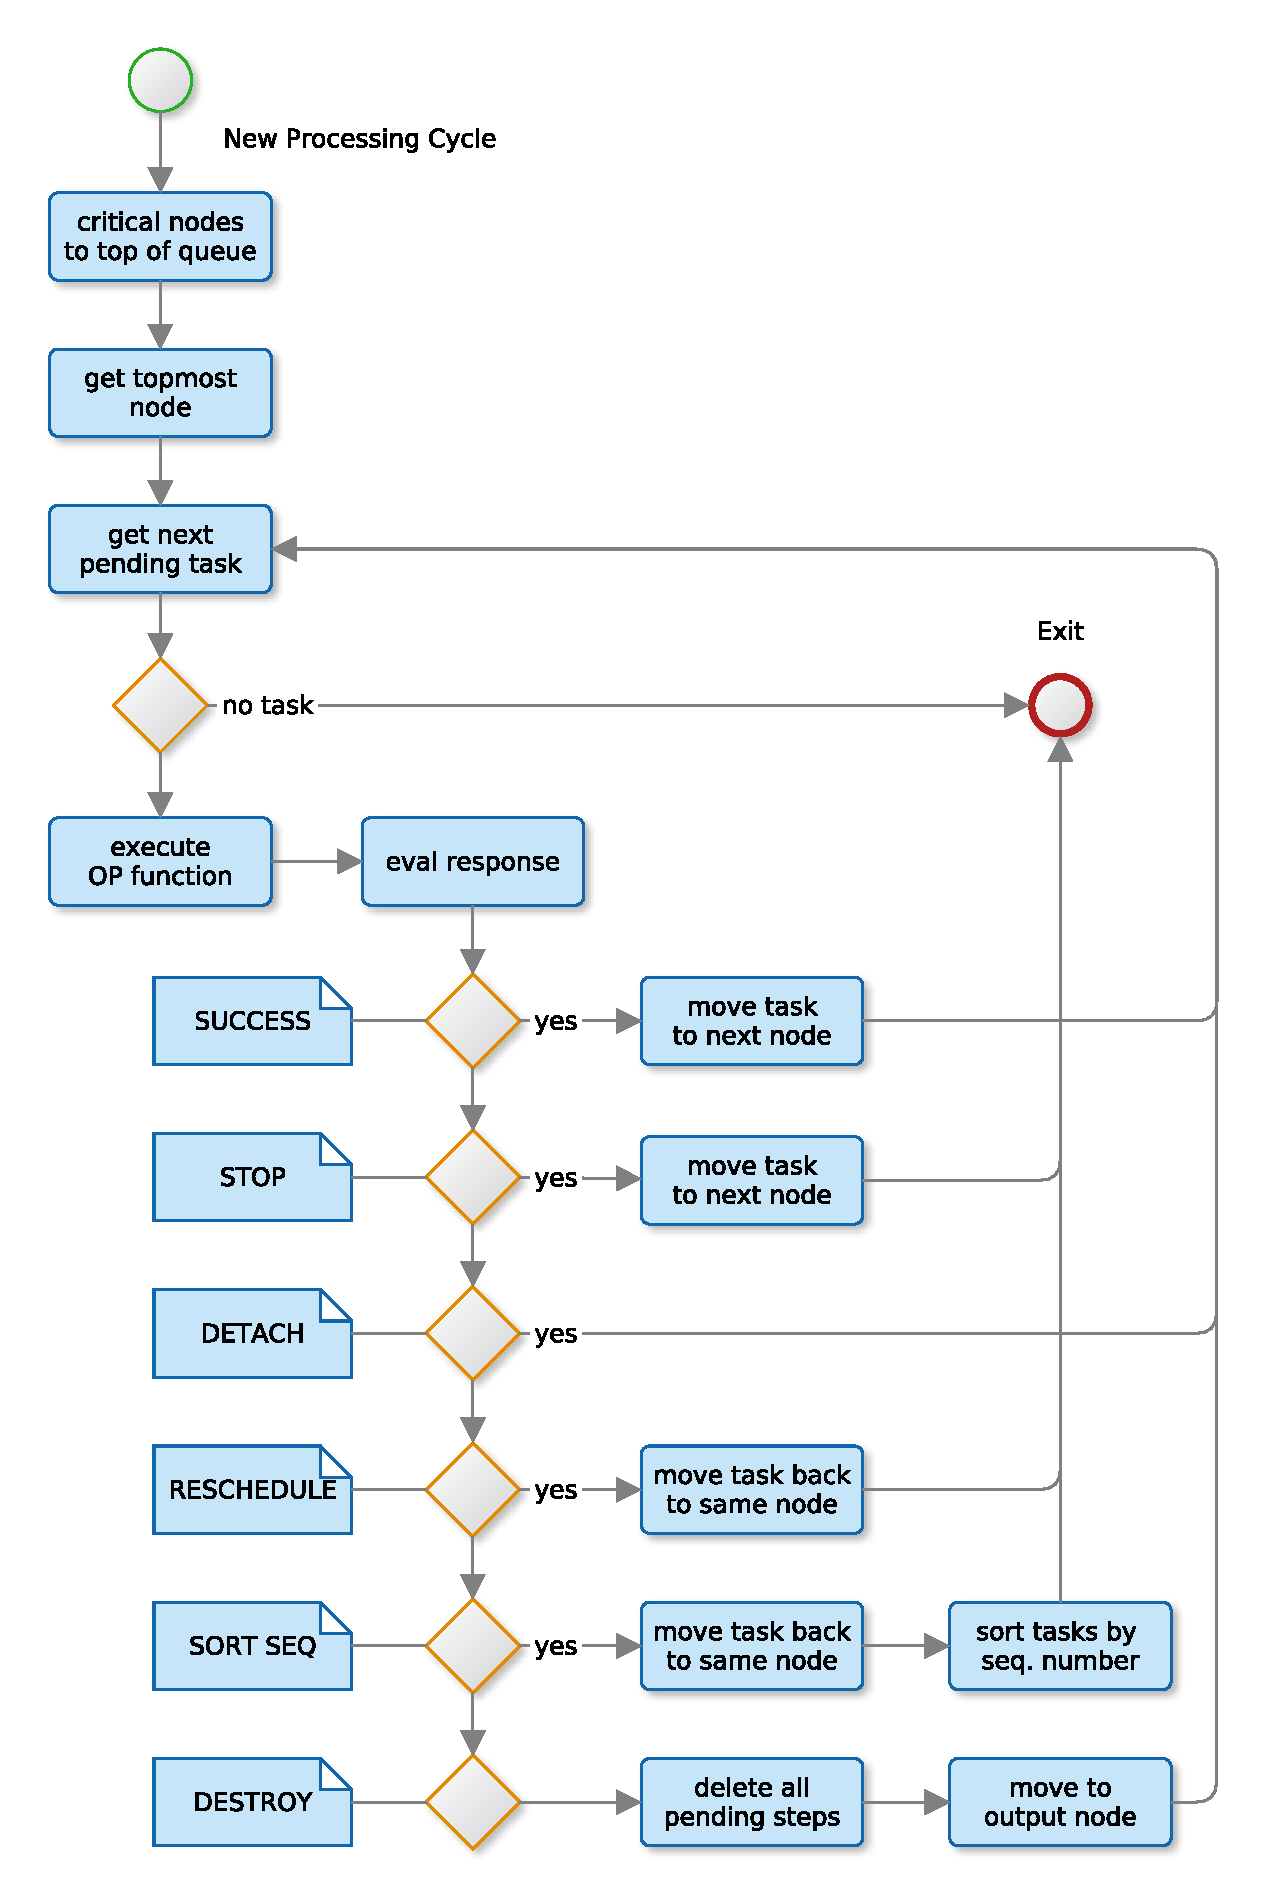
\includegraphics[width=0.8\columnwidth]{images/proc_network}
	\caption{A cycle of the processing network identifies possible critical
	tracker nodes and moves them to the top of the queue. The top-most
	tracker on the node stack is then processed until abort is commanded,
	or the tracker input is empty. Processed tasks are propagated to
	the next matching node in their processing step list.}
	\label{fig:proc_network}
\end{center}
\end{figure}


Processing tracker nodes do not handle task management themselves. Instead,
they are part of a network that propagates the tasks between the nodes.
When a task is added to the input of a network, it inspects the op code of the first
item of the task's step list and moves the task to the input of a matching
tracking node.
\\

The execution cycles of tasks are controlled by the user. To execute the input
tasks on any tracker, a function is called to initiate a processing cycle
(\fig{fig:proc_network}). The network then looks for trackers above their
critical threshold and moves them to the top of the execution queue in any
order and executes the top-most item of the stack. If no critical trackers are
present, the first non-empty tracker encountered is executed. The return code
of the executed operation is then evaluated.  For each processed task, the
processing step list is updated by moving the top-most op code (which was just
executed) to the DONE list and the task is forwarded to the matching
tracker of the next pending op code on its TODO list. This process is
repeated until the input of a tracker is empty, or task processing abort is
signalled by a return code of the operator function.

Once all steps on a task's processing list are completed, it is moved to the
output node of the network, which executes a user-defined function that takes
care of any further treatment of the task, e.g. to move it to mass memory.
\\

Processing functions may arbitrarily manipulate a task. This includes deletion
or addition of steps, change of data buffers and so on. A processing function
may even collect a number of tasks, merge their data (e.g. by performing an
image stacking operation), then re-add the newly shaped task to back to the
network and destroy the remaining, now empty tasks.
\\

If an operation is to be applied multiple times or recursively (e.g. for
wavelet decomposition), the pending step list can contain multiple entries of
the same \emph{op code} (\fig{fig:task_network}).
\\

This characteristic can also be used to very easily construct state machines,
where the processing function control the state machine transitions by
manipulating the processing step list until certain conditions are met.



\section{Building a Generic Processing Network}

The Xentium processing network is based on the generic implementation of a
processing network, which may be used to create, develop and representatively
test processing operations before their implementation in Xentium kernel
programs.
\\

\noindent
A processing network consists of a number of processing trackers, each having
an \emph{op code} and an a corresponding function assigned. The trackers define
a critical level of pending tasks, which is used for priority scheduling.

Pending items are tracked as doubly-linked lists, where each item provides the
storage space of the links itself. This means that, while nodes may reach a
\emph{critical fill level}, they can never run out of memory space.
\\

\noindent
A processing network is created by calling:

\begin{lstlisting}
	struct proc_net *pn = pn_create();
\end{lstlisting}

\noindent
Then to add a task tracker that acts as a processing node, we must define a
function with a matching interface. A simple example is a function
that just increments all data by one:

\begin{minipage}{\linewidth}
\begin{lstlisting}
int op_inc(unsigned long op_code, struct proc_task *t)
{

	size_t i;
	size_t n;

	unsigned int *p;


	/* get the number of datums */
	n = pt_get_nmemb(t);

	/* get the data buffer associated with this task */
	p = (unsigned int *) pt_get_data(t);

	/* n is not 0, but data is NULL, this task is malformed and
	 * will be moved directly to the output node with all
	 * elements set to zero
	 */
	if (!p)	
		return PN_TASK_DESTROY;

	/* increment all items by 1 */
	for (i = 0; i < n; i++)
		p[i]++;

	/* signal successful completion */
	return PN_TASK_SUCCESS;
}
\end{lstlisting}
\end{minipage}

\noindent
Such functions may return a variety of status code, please refer to the
API description in the source files or the documentation generated from the
\gls{Doxygen} markup.
\\

\noindent
The \emph{op\_inc} function is then registered as a new tracker, with the op
code \emph{0x12345678} and a critical level of \emph{5} and added to the
processing network:

\begin{lstlisting}
	pt = pt_track_create(op_inc, 0x12345678, 5);
	pn_add_node(pn, pt);
\end{lstlisting}

\noindent
Similarly, we could create more nodes, for example to decrement and multiply:

\begin{lstlisting}
	struct proc_tracker *pt = pt_track_create(op_dec, 0x22225555, 10);
	pn_add_node(pn, pt);

	pt = pt_track_create(op_mul, 0x00000bad, 2);
	pn_add_node(pn, pt);
\end{lstlisting}

\noindent
Finally, we must create an output node, otherwise the processing network
would just keep accumulating fully processed tasks.

\begin{minipage}{\linewidth}
\begin{lstlisting}
int op_output(unsigned long op_code, struct proc_task *t)
{
	size_t i;
	size_t n;

	unsigned int *p;



	n = pt_get_nmemb(t);
	p = (unsigned int *) pt_get_data(t);

	/* print the result */
	if (p) {
		for (i = 0; i < n; i++) {
			printk("\t%d\n", p[i]);
		}
	}

	/* deallocate the data buffer */
	kfree(p);

	/* destroy the task */
	pt_destroy(t);

	return PN_TASK_SUCCESS;
}
\end{lstlisting}
\end{minipage}

\noindent
The output node is special in that its \emph{op code} is zero and it should 
be used to deallocate the data buffer, which is not automatically done by
\emph{pt\_destroy()}, as the management of this buffer is solely the
responsibility of the user.


\begin{lstlisting}
	pn_create_output_node(pn, op_output);
\end{lstlisting}

\noindent Now that the processing network is defined, we may add tasks. Here we
create a task and assign it  a data buffer that holds \emph{32} bytes and at
most \emph{4} processing steps. The type and sequence number fields are not
used and simply set to zero. The number of elements in the buffer is then set
to \emph{5}, assuming it has been prepared accordingly.

\begin{lstlisting}
	struct proc_task *t = pt_create(data, 32, 4, 0, 0);

	pt_set_nmemb(t, 5)
\end{lstlisting}


\noindent In order to define the sequence of processing steps we want to be
performed on our data buffer, we now configure them in the desired order and
the proper op codes:

\begin{lstlisting}

#define OP_INC 0x12345678
#define OP_DEC 0x22225555 
#define OP_MUL 0x00000bad

	pt_add_step(t, OP_INC, NULL);
	pt_add_step(t, OP_INC, NULL);
	pt_add_step(t, OP_MUL, NULL);
	pt_add_step(t, OP_DEC, NULL);

\end{lstlisting}

\noindent
Note how we added \emph{OP\_INC} twice. This will result in that operation
being applied twice in row, as the task is moved into the next node after
processing the first step, which happens to be the identical node
it just went through. This may be used to define multiple passes and recursion.

As the op functions may also manipulate the processing step list of a task
arbitrarily, this can also be used to easily create state machines.
\\

\noindent
Note that steps with invalid \emph{op codes}, i.e. those for which no tracker
node has been registered will result in the destruction of the task as if
an \emph{op function} had returned \emph{PN\_TASK\_DESTROY}
\\

\noindent
The task is the added to the input node of the network:

\begin{lstlisting}
	pn_input_task(pn, t);
\end{lstlisting}

\noindent
This does not yet start processing, as the network input and output rates are
user controlled. To trigger processing of the tasks pending in the input node,
we call:

\begin{lstlisting}
	pn_process_inputs(pn);
\end{lstlisting}


\noindent
Tasks processing cycles are then executed by repeatedly calling:

\begin{lstlisting}
	pn_process_next(pn);
\end{lstlisting}

\noindent
which will result in the execution of a single task step of a single node.
If one of the tracker nodes is above it's critical threshold, it will be
processed instead of the last tracker, otherwise the last tracker is processed
until its pending tasks list is empty.
\\

\noindent
To process the acumulated tasks in the output node we call:

\begin{lstlisting}
	pn_process_outputs(pn);
\end{lstlisting}

\noindent
which will result in the execution of the user defined output function for
one pending output task per call.
\\

\noindent
Note that in case of the Xentium processing network, the call to
\emph{pn\_process\_next()} and the input processing trigger is controlled by
the driver and user control is only needed to execute a processing cycle on the
output node.

\section{Building a Xenitum Processing Network}


The specific implementation of the Processing Network on the Xentium DSPs maps
\emph{op codes} to Xentium programs instead of C functions. These programs
are added to the Xentium driver by calling

\begin{lstlisting}
	xentium_kernel_add(file);
\end{lstlisting}

\noindent
where \emph{file} is a pointer to a memory buffer holding the ELF executable
of a Xentium program. As the driver loads the file, it reads a static structure
defined in the program, that contains information on the capabilities of the
kernel (see \emph{dsp/xentium/kernels/} for examples). The driver then registers
a processing tracker node for this particular program kernel and adds it to the
network. Alternatively, DSP programs may be auto-loaded from the AR archive
file \emph{modules.image} embedded in the executable. During the build process
of the operating system image, all files with a suffix of \emph{.xen} in the
\emph{dsp/} source tree are automatically added to this archive. To add all
of these executables to the network, one can simply call:

\begin{lstlisting}
	module_load_xen_kernels();
\end{lstlisting}

\noindent
To set up the processing network, an output node has to be added, as described
in the previous section:

\begin{lstlisting}
	xentium_config_output_node(op_output);
\end{lstlisting}

\noindent
Now tasks may be created (see above) and added to the Xentium processing network
via the call:

\begin{lstlisting}
	xen_new_input_task(t);
\end{lstlisting}

\noindent
This will also take care of calling \emph{pn\_process\_inputs()} that had
to be done by the user in the generic function based implementation described
earlier.
\\


\noindent
As before, the user must call for outputs to be processed. This is done by:

\begin{lstlisting}
xentium_output_tasks();
\end{lstlisting}


\section{Xentium Kernel Programs}

A Xentium kernel program is slightly more complex than the functions described
above, as it must also take care of memory management and NoC DMA programming.
\\

\noindent
First, it defines its own capabilites and, optionally, permanently assigned
system memory storage allocated by the driver:

\begin{lstlisting}
#define KERN_NAME		"example"
#define KERN_STORAGE_BYTES	128
#define KERN_OP_CODE		0x0000000a
#define KERN_CRIT_TASK_LVL	0x5

struct xen_kernel_cfg _xen_kernel_param = {
	KERN_NAME, KERN_OP_CODE,
	KERN_CRIT_TASK_LVL,
	NULL, KERN_STORAGE_BYTES,
};

\end{lstlisting}

\noindent
This structure is found in \emph{include/kernel/xentium\_io.h}. It defines
the Xentium kernel's name, the number of storage bytes, its op code and critical
threshold of input tasks. As the driver loads the executable, it analyses the
structure parameters and creates and registers a processing node accordingly.
If the kernel requests a permanent storage (128 bytes in this example), the
driver allocates a suitable memory buffer and patches its address in the
executable's corresponding ELF symbol record.
\\

\noindent
Next, the program kernel needs a main function, which is very generic and
consists of a simple loop that parses the messages sent by the driver:

\begin{minipage}{\linewidth}
\begin{lstlisting}
int main(void)
{
	struct xen_msg_data *m;

	while (1) {
		m = xen_wait_cmd();

		switch (m->cmd) {
		case TASK_EXIT:
			/* confirm abort */
			xen_send_msg(m);
			return 0;
		default:
			break;
		}
		process_task(m);

		xen_send_msg(m);
	}

	return 0;
}

\end{lstlisting}
\end{minipage}

\noindent
Here it waits for the host to write a message into its designated command
mailbox. If the command is to exit, it confirms by responding with the identical
message, otherwise it calls its processing function and then relays the message
set by the latter back to the host.
\\

\noindent
A processing function that simply copies a number of bytes to and from the
Xentium's \gls{TCM} via the \gls{NoC} \gls{DMA} is shown below:

\begin{minipage}{\linewidth}
\begin{lstlisting}

static void process_task(struct xen_msg_data *m)
{
	size_t n;

	unsigned int *p;
	volatile unsigned int *b1;

	struct xen_tcm *tcm_ext;


	b1 = (volatile unsigned int *) xen_tcm_local;



	if (!m->t) {
		m->cmd = TASK_DESTROY;
		return;
	}

	tcm_ext = xen_get_base_addr(m->xen_id);


	n = pt_get_nmemb(m->t);
	p = pt_get_data(m->t);


	if (n > XEN_TCM_BANK_SIZE / sizeof(unsigned int))
		n = XEN_TCM_BANK_SIZE / sizeof(unsigned int);

	/* retrieve data to TCM */
	xen_noc_dma_req_lin_xfer(m->dma, p, tcm_ext, n, WORD, LOW, DMA_MTU);

	/* no processing */

	/* back to main memory  */
	xen_noc_dma_req_lin_xfer(m->dma, tcm_ext, p, n, WORD, LOW, DMA_MTU);


	m->cmd = TASK_SUCCESS;
}

\end{lstlisting}
\end{minipage}

\noindent
With the exception of the \gls{DMA} access and message exchange instead of return
codes, the structure of such a function is very similar to a non-DSP op function
in how it accesses the data contents of the processing task.
In addition, it must also take care of data exchange between remote system
memory and the \gls{TCM} to achieve proper perfomance.
\\

\noindent
This kernel program can then be added to \emph{dsp/xentium/kernels/} and
\emph{dsp/xentium/Makefile} must be edited to include the program in the
build process.



\chapter {Custom Xentium DSP Assembly}

\section{Overview}

With an architecture like the \gls{Xentium}, compilers have a hard time
optimising for instruction parallelism, hence the ``human code generator'' is
still most effective in designing efficient implementations. \\

While assembly is usually a subject that tends to intimidate many programmers,
the simplicity and straightforwardness of the Xentium assembly
language\cite{XenUsrGuide} along with the architectural concept of the DSP
registers and functional units, makes it easy to grasp and use once a certain
level of familiarity has been established. \\

Still, the design of what are mostly functionally sequential, but very often
data parallel algorithms, such as in AlgoLib, requires a certain level of
twisted thinking, as this is usually not how our minds work.  To help oneself,
one must conceive a method to facilitate the development of such tasks, one
which will presented here. \\

Please note, that this chapter \emph{does not} intend to teach how to write
Xentium assembly, but merely demonstrates a method that can be very useful
approach in development.


\section{Rampfit Optimisation Example}


\begin{minipage}{\linewidth}
\begin{lstlisting}
/* author: R. Ottensamer */
int FastIntFixedRampFitBuffer(long *data, unsigned int n_samples,
			      unsigned int ramplen, long *slopes)

{
	int i      = 0;
	int r      = 0;	
	int ampl   = ramplen;
	int SyTerm = 0;
	int pos    = 0; /* temporary offset storage */
	int value  = 0; /* temporary sample storage */

	int Sy;
	int Sxy;


	for (pos = 0; pos < (n_samples - ramplen + 1); )
	{
		Sy  = 0;
		Sxy = 0;

		for (i = 1; i <= ramplen; i++) /* equation starts with 1 */
		{
			value = data[pos++];
			Sy   += value;
			Sxy  += i * value;
		}

		SyTerm      = ampl * ((ramplen + 1) * Sy) >> 1;
		slopes[r++] = ampl * Sxy - iSyTerm;
		/* denomination has to be done outside */
	}

	return r;
}
\end{lstlisting}
\end{minipage}

\noindent
Let us consider the the above example of a fast ramp fitting routine. Looking
at the inner loop, we can immediately spot one load operation, three additions,
and one multiplication.  We can put pos++ anywhere after the load, but the
operations

\begin{lstlisting}
[load] - [add,mul] – [add]
\end{lstlisting}

\noindent must occur in this sequence. Note that the operations that can be
executed in parallel are already grouped by brackets. \\

\noindent Now, this is actually incorrect, because the results of \emph{load}
and \emph{mul} are not available in the next cycle, so we introduce a
\emph{[wait]} tag:

\begin{lstlisting}
[load] - [wait] – [add Sxy,mul value] – [wait] – [add Sxy]
\end{lstlisting}

\noindent
This actually takes 5 cycles to complete. There are lots of inactive
units, so instead of loading one word, we'll load two and increment the missing
\emph{pos++} (we need one per sample) in the first free cycle:

\begin{lstlisting}
[load1,load2] – [pos1,pos2] – [Sy1,Sy2,mul1,mul2] – [wait] – [Sxy1,Sxy2]
\end{lstlisting}

\noindent
So we doubled our processing speed, but there are still lots of inactive units.
We can actually load 4 words at once, using 2 \emph{E} units, so let's try that:

\begin{lstlisting}
[load1,load2,load3,load4]-[wait]–[add1,add2,add3,add4,mul1,mul2,mul3,mul4] – [wait] – [...]
\end{lstlisting}


\noindent
This is getting complicated, and we're out of \emph{M} units.
Let's try to rewrite this:




\begin{lstlisting}
|load1||pos1++||add 1,2||mul3     ||add mul1,mul2||add mul3,mul4||add m12,m34|
|load2||pos2++||add 3,4||mul4     ||             ||             ||           |
|load3||pos3++||       ||add 12,34||             ||             ||           |
|load4||pos4++||       ||         ||             ||             ||           |
|     ||      ||mul1   ||         ||             ||             ||           |
|     ||      ||mul2   ||         ||             ||             ||           |
\end{lstlisting}

\noindent
We managed to process 4 samples in 7 cycles instead of 2 in 5 (second try) or 1
in 5 (first try), so we're down to 1.75 cycles per sample instead of 5, that's
a speed-up of \approx 2.85x. \\

\noindent
Not bad. But there are still many unused units per cycle. And we're still
missing a lot of other code, this is actually only the three lines of the inner
loop. Besides, constructing the assembly in this manner is really tedious.
Luckily, this can be helped. \\

\begin{figure}
\begin{center}
	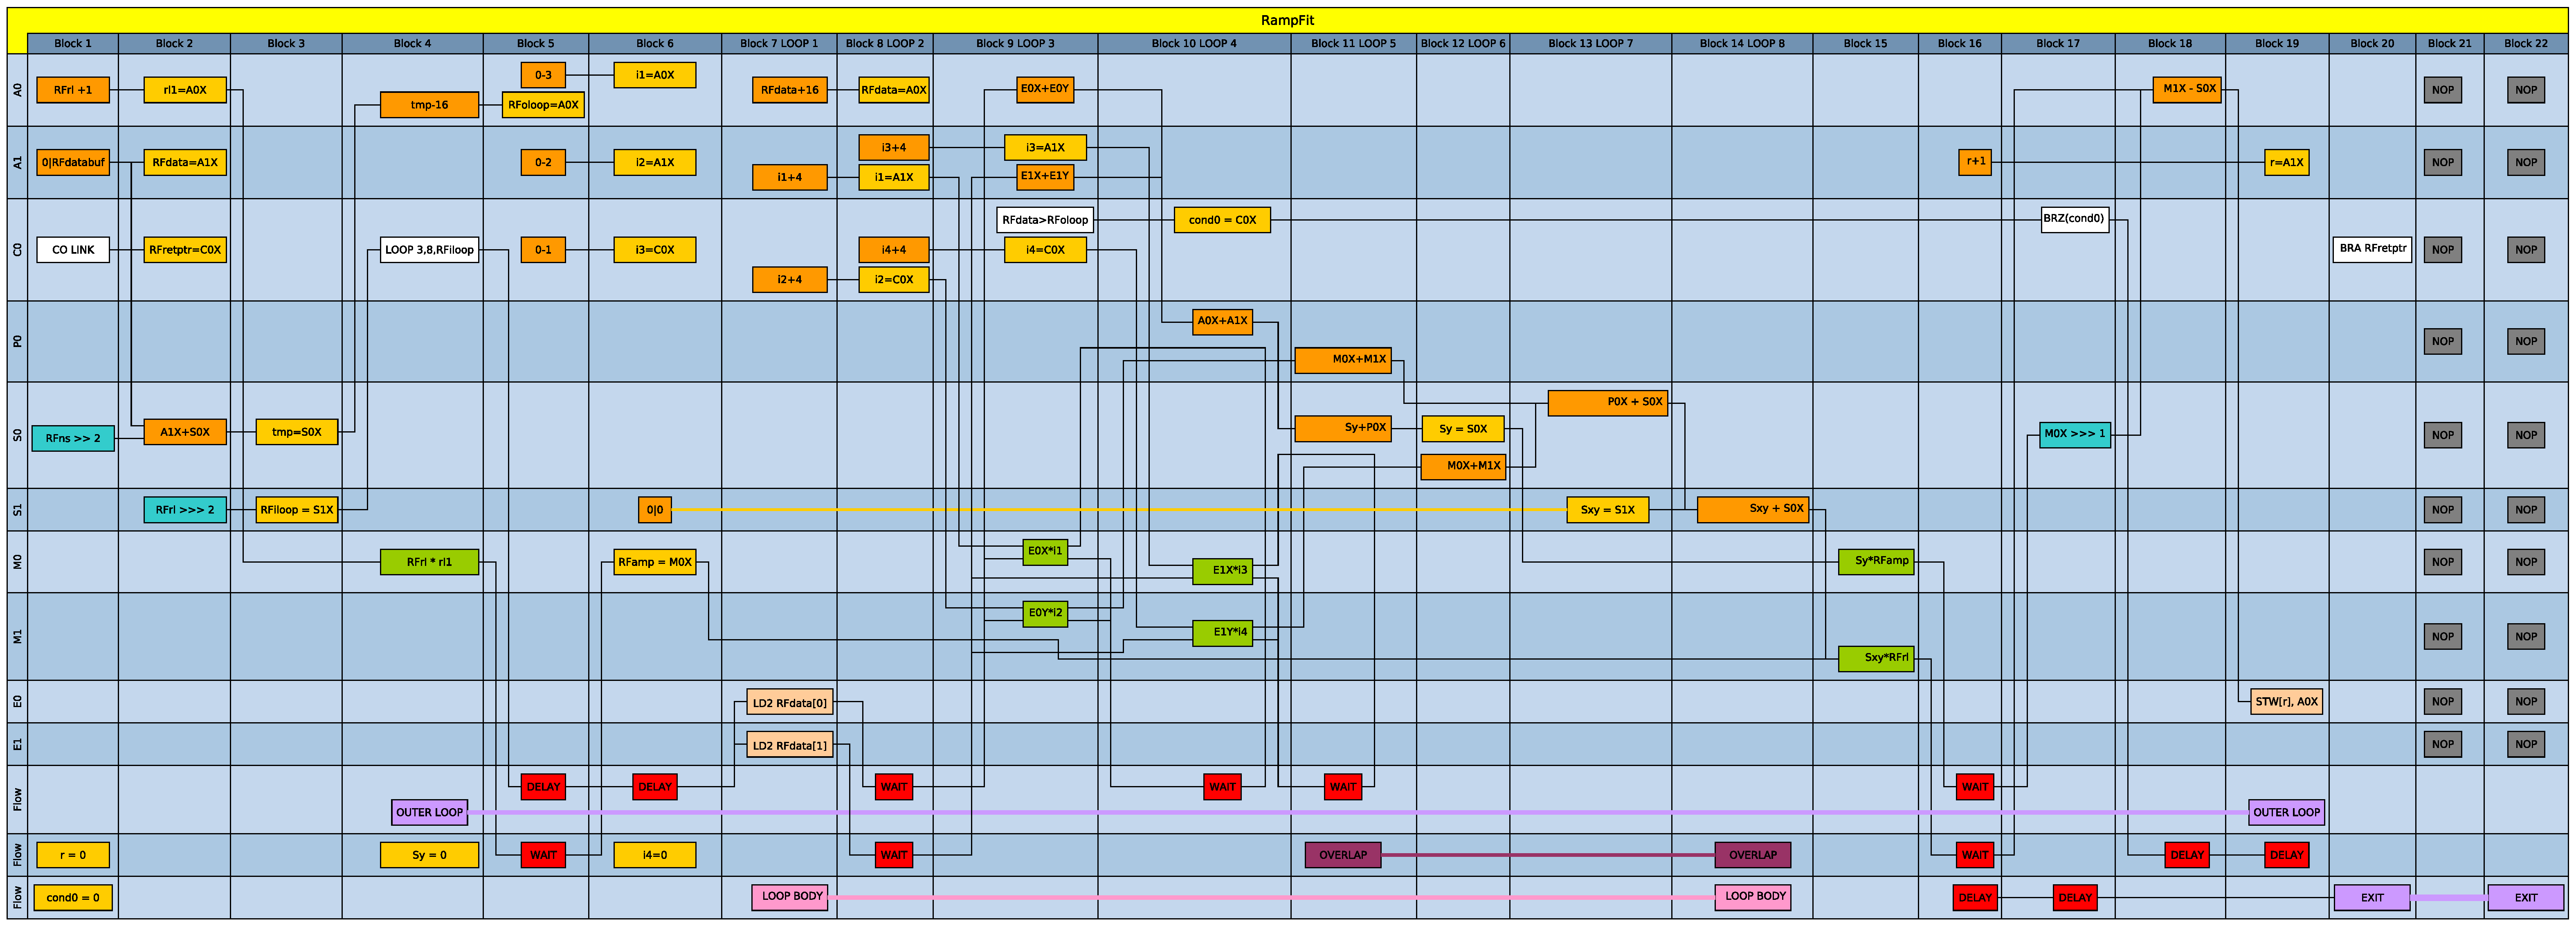
\includegraphics[width=1.0\columnwidth]{images/rampfit_xen}
	\caption{A swimlane graph of the rampfit in parallelised Xentium
		assembly (symbolic).}
	\label{fig:xenramp}
\end{center}
\end{figure}

\noindent
It turns out that this is best done in a diagramming program with swim lane
support (\fig{fig:xenramp}), such as \emph{yEd}: \\

\noindent
Create 10 swim lanes to represent the functional units, along with a few lanes
for flow tags, such as

\begin{lstlisting}
 [wait] or [delay]
\end{lstlisting}

\noindent
Add an arbitrary number of columns to represent cycles. \\

\noindent
Insert one operation per cycle and swim lane and connect the processing steps
for reference, and remember to insert delays and wait states when they occur.
In addition, add special tags to outline register write operations, so the
location of variables can be tracked. \\

\noindent
Using this method, the ramp fit example above can be tuned even more, down to
to a processing time of 0.75 cycles per sample, not including overhead (see
listing below). Obviously not all algorithms need this kind of
optimisation, but this one benefits a lot with greater than 6.5x speed-up over
the serial version, as it is usually applied to large datasets. In addition it
is a great showcase of the potential of the Xentium DSP, especially regarding
the hardware LOOP support, which allows us to efficiently schedule repetitive
instructions in parallel by “overlapping” instruction blocks. This is
demonstrated in the listing below, where the instruction blocks in loop body
block 1-3 start being executed in parallel starting with block 4. \\\\


\begin{lstlisting}
.globl FastIntFixedRampFitBuffer
.align 4
.type FastIntFixedRampFitBuffer,@function

;; input data length must be a multiple of 4!

;; function call arguments
%define RFdatabuf1	RA6
%define RFdatabuf2	RB6
%define num_samples	RC6
%define ramp_len	RD6
%define RFslopebuf	RE6
;; reserved registers
%define RFretptr 	RA7
%define RFretval 	RA6
%define cond0		RC0
%define cond1		RB0

;; constants and local variables
%define RFdata1		RA5
%define RFdata2		RC2
%define rl1        	RC5 
%define Sy		RE2
%define Sxy		RD5
%define r		RA6
%define RFiloop	RE1
%define tmp		RA4

%define RFoloop	RD4

%define i1		RA2
%define i2		RB2

%define i3		RC3
%define i4		RD3
%define RFamp	RE3

FastIntFixedRampFitBuffer:
	;; block 1
	A0 ADD  ramp_len, 1	; calculate ramplen +1 = rl1
	A1 OR   0, RFdatabuf1	; RFdata1
	S1 OR   0, RFdatabuf2	; RFdata2
	C0 LINK
	S0 SL   num_samples, 1		; RFns * 4 / 2 = offset to end of buffer in words, split into two banks
	cond0 = 0		
	r     = 0
	
	;; block 2
	S0 ADD A1X, S0X		; end of buffer 
	S1 SRU ramp_len, 2		; RFiloop = ramp_len/4 
	rl1      = A0X
	RFdata1  = A1X
	RFdata2  = S1X
	RFretptr = C0X
	
	;; block 3
	RFiloop = S1X
	tmp =  S0X
		
.RFloop:
	;; block 4
	C0 LOOP 3, 8, RFiloop		
	M0 MUL  ramp_len, rl1		; RFamp  - compute every time, saves 1 cycle during lead in plus unit is free anyway
	A0 SUB tmp, 8			
	Sy = 0
	
	;; block 5; loop delay slot 1
	A0 SUB 0, 3		; i1	prepare indices with negative offset
	A1 SUB 0, 2		; i2	before entering the loop, they are
	C0 SUB 0, 1		; i3    incremented to 1,2,3,4 on the first pass
	RFoloop = A0X
	

	;; block 6; loop delay slot 2
	S1 OR 0, 0			; prep initial Sxy (need that to properly fold the loop)
	RFamp = M0X
	i1    = A0X
	i2    = A1X
	i3    = C0X
	i4    = 0
	
	;; block 7; loop body block 1
	A0 ADD RFdata1, 8		; forwared 2 samples (words)
	A1 ADD i1,  4			; increment loop indices
	C0 ADD i2,  4
	E0 LD2 RFdata1			; load from current
	E1 LD2 RFdata2

	;; block 8; loop body block 2
	A0 ADD RFdata2, 8		; forward 2 samples
	A1 ADD i3,  4			; increment loop indices
	C0 ADD i4,  4
	i1  = A1X			; update loop indices
	i2  = C0X
	RFdata1 = A0X			; updated buffer1 pointer
	
	;; block 9; loop body block 3
	A0 ADD E0X, E0Y			; sum first pair
	A1 ADD E1X, E1Y			; and second pair
	M0 MUL E0X, i1			; multiply first two samples with
	M1 MUL E1X, i2			; loop index
	C0 CMPGT RFdata1, RFoloop	; check if we reached end of buffer
	i3   = A1X			; update loop indices
	i4   = C0X
	RFdata2 = A0X			; updated buffer2 pointer

	;; block 10; loop body block 4
	P0 ADD A0X, A1X			; final sum of all samples
	M0 MUL E0Y, i3			; multiply 3rd and 4th sample with loop
	M1 MUL E1Y, i4			; index
	cond0 = C0X			; update result of condition
	
	;; block 11; loop body block 5
	S0 ADD Sy,  P0X			; add sum of 4 samples to Sy
	P0 ADD M0X, M1X			; add result of first two samples * loop idx

	;; block 12; loop body block 6
	S0 ADD M0X, M1X			; add result of 3rd and 4th sample * loop idx
	Sy = S0X			; assign new Sy
	
	;; block 13; loop body block 7
	S0 ADD P0X, S0X			; final sum of idx * sample multiplications	
	Sxy = S1X			; update Sxy from previous cycle

	;; block 14; loop body block 8
	S1 ADD Sxy, S0X	 		; add new idx * sample to Sxy
		
	;; block 15 - back in outer loop (the inner loop ends automatically)
	M0 MUL Sy,  RFamp		; mulitply Sy with amplifier
	M1 MUL S1X, ramp_len		; use latest Sxy and multiply with ramplen (ampl)

	;; block 16 - wait 
	A1 ADD r, 1			; increment number of ramps processed 

	;; block 17
	C0 BRZ, cond0 .RFloop		; init branch to start of outer loop
	S0 SRU M0X, 1			; divide iSyTerm

	;; block 18	
	A0 SUB M1X, S0X			; calculate slope

	;; block 19 - BR delay slot 1
	E0 STW RFslopebuf[r], A0X	; A0X from block 18
	r = A1X				; update r (in loop) ; RFretval == r!

	;; block 20 - BR delay slot 2
	C0 BRA RFretptr			; init branch back to caller

	;; block 21+22
	NOP 2				; final delay slots

	;; Elvis has left the building
\end{lstlisting}




\appendix
\chapter {Changes from NGAPP to LeanOS Xentium Processing Concept}

The following sections look at the major differences between the NGAPP and
LeanOS concepts.

\section {Processing Chain}

In contrast to the implementation of the Xentium processing chain for
\gls{NGAPP}, a processing chain is not set up statically but defined
individually on a per-task basis by selecting from a set of processing kernel
nodes. Each of these nodes define their own capabilities as an \emph{op code},
which is used to construct a proccessing chain on-the-fly on a per-task basis.


\section {Input buffering}

Contrary to the fixed-size circular input buffers originally used in \gls{NGAPP}
processing chain design, pending items are now tracked as doubly-linked lists,
where each item provides the storage space for the links itself. This means
that, while nodes may reach a \emph{critical level}, they can never run out of
memory space.



\end{document}
